\subsection{YANA Core Architecture}
YANA is a digital \ac{SNN} emulator, as all of its logic and memory resources are dedicated either to implementing neurosynaptic operations or to transporting events. Furthermore, YANA is an event-driven processor; it only processes events once they arrive and is otherwise idle. It implements a near-memory processing pipeline that encapsulates multiple neurons and synapses. The neurons and synapses share the same processing logic within the core in time-multiplexed fashion, which reduces resource utilization~\cite{frenkel_bottom-up_2023}. Furthermore, processing and communication resources operate concurrently -- neuron state updates, spike emission and spike transport all occur in parallel within a timestep.
\begin{figure*}
  \centering
  \makebox[\textwidth]{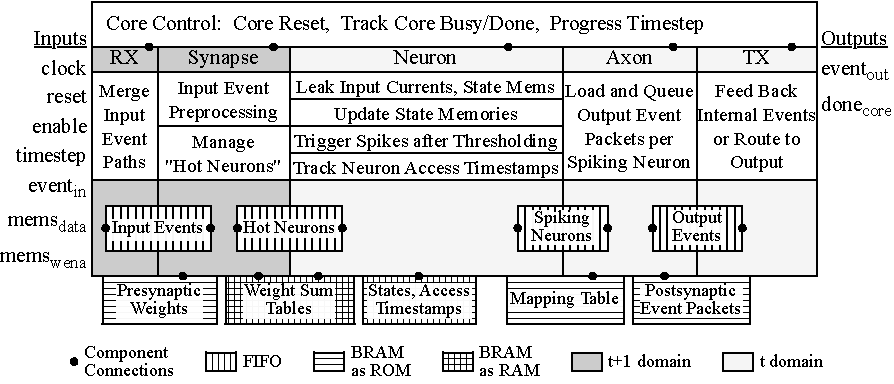
\includegraphics[width=0.95\textwidth]{media/YANA_core_block_diagram.pdf}}
  \caption{High-level block diagram of the YANA core.}
  \label{YANA-core-block-diagram}
\end{figure*}
The core's processing pipeline consists of five main stages as depicted in Figure~\ref{YANA-core-block-diagram}. The stages are briefly described as follows:
\begin{itemize}
  \item \textbf{Input Stage (RX):}
  The input stage receives events from two possible stream sources, either from the external interconnect or from the core's internal feedback path.
  \item \textbf{Synapse Stage:}
    The synapse stage preprocesses input events on arrival. The preprocessing results in pre-synaptic weight sums for each neuron, which are stored in dedicated BRAMs. The synapse stage also tracks which neurons have received at least one event in the current timestep, storing this information in the Hot Neurons FIFO.
  \item \textbf{Neuron Stage:}
    The neuron stage updates the states of all hot neurons and queues spiking neurons for spike emission in the axon stage. It currently implements a Forward-Euler \ac{LIF} neuron model, through which state updates caused by leak can be deferred to the arrival time of the next event.
  \item \textbf{Axon Stage:}
  In the axon stage, each spiking neuron triggers the loading and emission of its associated list of post-synaptic events. The amount of post-synaptic connections is programmed per-neuron in a mapping table.
  \item \textbf{Output Stage (TX):}
  For each emitted event, the output stage checks whether the event is destined for a synapse within the core or for an external destination, branching it to the internal feedback path or the external interconnect, respectively. 
\end{itemize}

\noindent The following sections detail key aspects of YANA's implementation:
\\
\textbf{Timestep Progression Scheme:}
The core operates in discrete timesteps and derives the progression of timesteps from its input event workload. Each stage in the processing pipeline sets a load-dependent idle signal that is read by the core's local control logic. Once the whole pipeline is idle, the control logic sets the signal $core_{done}$, which signifies that the core is ready to progress to the next timestep.
Ultimately, an external layer of control logic is responsible for progressing the core's input signal $timestep$, depicted in Figure~\ref{YANA-core-block-diagram}.
In this work's evaluation, we implement timestep progression logic for the use case of processing neuromorphic datasets. Dedicated control logic reads timestamps from the dataset sample's events and progresses the timestep 
accordingly, without any downtime related to elapsed wall time; depending on the workload, this enables faster-than-realtime processing.
\\
\textbf{Input Event Preprocessing Scheme:}
The discretization of timesteps in \acp{SNN} requires that each event is assigned to a specific timestep for processing. YANA's synapse stage preprocesses arriving
input events to completely avoid raw input event buffering while maintaining a steady input rate of $1\nicefrac{\text{event}}{\text{cycle}}$. As events arrive, the synapse stage continuously integrates the associated weights into per-neuron weight sums. A weight sum represents the total (unleaked) input current that will be added to the respective neuron's membrane potential in
the next timestep.
\\
\textbf{Event-driven Neuron Updates:}
YANA updates neuron states only once they are \textit{hot}, that is, once they have received at least one event in the current timestep. This applies both to integrating input currents and to processing continuous leak dynamics. To this end, the neuron stage implements the forward Euler solution of the \ac{LIF} neuron model:
\begin{equation}
  \label{eq:lif_update}
  \tilde{u}(t+n) = u(t) \cdot \left(1 - \frac{1}{\tau_{\text{mem}}}\right)^n + \frac{1}{\tau_{\text{mem}}} \cdot i(t)
\end{equation}
\begin{equation}
  \label{eq:lif_spike_condition}
  u(t+n) = \begin{cases}
    \tilde{u}(t+n) & \text{if } \tilde{u}(t+n) \leq u_{\text{th}} \\
    0 & \text{if } \tilde{u}(t+n) > u_{\text{th}} \text{ (spike occurs)} \\
    0 & \text{if } n > n_{\text{max}} \text{ (round to 0)} \\
  \end{cases}
\end{equation}
In the equations, $u(t)$ is the neuron's membrane potential at timestep $t$, $I(t)$ is the neuron's input current at timestep $t$, and $\tau_{\text{mem}}$ is the membrane time constant. The parameter $n$ represents the number of timesteps that have passed since the last update of the neuron's state. $\tilde{u}(t+n)$ is a temporary variable that holds the result of the leak and input current integration. In YANA, the equations are fully implemented using fixed-point arithmetic.

Note that only the leak term $(1 - \nicefrac{1}{\tau_{\text{mem}}})^n$ depends on the time that has passed since the last neuron update. To efficiently implement this calculation, the neuron stage uses a \ac{LUT} with precalculated solutions to this term for $n_{\text{max}}$ entries, thereby eliminating the need to calculate the power function in hardware. If more than $n_{\text{max}}$ timesteps have passed since the last update, the neuron's membrane potential is rounded to 0 as shown in the second equation.

To support these deferred neuron updates, the neuron stage also maintains a record of the last access-timestamp for each neuron. This enables the core to calculate the number of elapsed timesteps $n$ when a neuron becomes hot, ensuring the correct application of the leak dynamics.
\\
\textbf{Support for Arbitrary SNN Graphs:}
YANA supports arbitrary SNN graphs by implementing point-to-point connections between pairs of neurons in its hardware architecture. The core maintains both pre-synaptic and post-synaptic information in separate memory structures. Pre-synaptic weights are stored in the synapse stage and accessed during event preprocessing, while post-synaptic destinations (dest.) are stored in connection tables accessed by the axon stage. Each outgoing connection is encoded as an event packet with the format:
\begin{equation*}
    \text{[ Dest. Core $(2bit)$ | Dest. Neuron $(10bit)$ | Dest. Synapse $(17bit)$ ]}
\end{equation*}
Since each event packet specifically addresses both target neuron and synapse, a single pre-synaptic weight in the synapse stage can be referenced by multiple connections, enabling native support for weight reuse and arbitrary pruning techniques. 

\subsection{System on Chip FPGA Integration}

\begin{figure}[t]
    \centering
    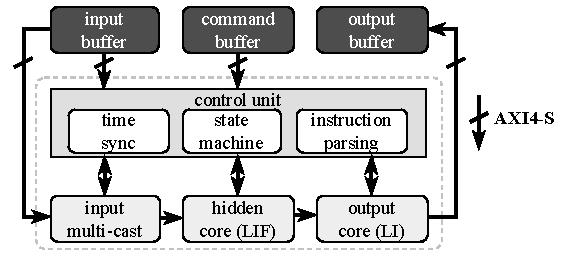
\includegraphics[width=0.7\textwidth]{media/YANA_experimental_setup.pdf}
    \caption{
    YANA architecture integration complete with AXI4 stream buffers, a control unit and cores for input, hidden and output computations.
    }
    \label{fig:exp_setup}
\end{figure}

In this work, we target the low-cost AMD Kria KR260 Robotics Starter Kit. The KR260 employs an AMD Zynq UltraScale+ \ac{SoC} FPGA which integrates software execution in its \ac{PS} and an adaptive FPGA fabric in its \ac{PL}.

As the YANA core architecture by itself only implements the pipelined data flow, there are additional components necessary in order to make it usable in an experimental setup, as can be seen in Figure~\ref{fig:exp_setup}.
To control the execution of the accelerator and communicate with the software stack, a \ac{CU} with a custom command interface is implemented. It keeps track of the global synchronized timestep, decodes and parses incoming commands and maintains an internal state machine to manage the control flow.
To interface with the accelerator's \ac{CU}, we instantiate AXI-enabled buffers for the input data, control commands and result output. These are accessible by the KR260's \ac{PS}, enabling runtime control of the accelerator from software.

Input events are source encoded, only containing information about the source input neuron and the timestep in which the input spike occurred. To multi-cast these input events to the destination encoded format expected by the hidden \ac{LIF} core, an input multi-cast core is integrated. Analogously, an output core containing \ac{LI} neurons integrates all spikes coming from the hidden core. Upon request, it returns the integrated neuron potential back to the \ac{PS} through the output buffer.

We use the previously mentioned dataset sample execution mode for the experiments conducted in this work, which involves loading entire samples into the input buffers of the accelerator and executing them as fast as possible until all input is processed.
After the execution of one sample finishes, the data path including any stateful memories is reset in preparation for the next sample.

\subsection{FPGA Resource Utilization}
Table~\ref{tab:resource-utilization} summarizes the resource utilization of a single YANA core and of the aforementioned experimental deployment on the KR260's \ac{PL}.
Our experimental deployment of YANA on the KR260 utilizes URAMs for storage of synaptic weights and event packets.
Synaptic parameters utilize the largest share of parameter storage in most applications; thus, URAMs are preferred over BRAMs to store them, if available.
Beyond FPGA resource utilization metrics, the table also specifies the resulting storage limits for mappable SNN parameters. YANA's \ac{RTL} design is thoroughly parameterized, and the \ac{SNN}-parameter storage limits are a result of configuring the desired number of synapses and neurons per core pre-synthesis, according to which synthesis infers the required amount of BRAM and URAM resources. Note that our experimental deployment of YANA in this work does not target application specific \ac{PL}-memory resource optimization. 
\begin{table*}
    \centering
    \resizebox{1\textwidth}{!}{
        \begin{threeparttable}
            \caption{FPGA resource utilization and available parameter storage of YANA core and experimental setup on KR260.}
            \label{tab:resource-utilization}
                \begin{tabular}{l*{5}{c}*{4}{c}} 
                    \toprule
                        \multirow{2}{*}[-2pt]{\textbf{Descriptor}} &
                        \multicolumn{5}{c}{\textbf{FPGA Resources}} &
                        \multicolumn{4}{c}{\textbf{Mappable Parameters}} \\
                    \cmidrule(lr){2-6} \cmidrule(lr){7-10}
                        & LUT & Register & BRAM\tnote{a} & URAM & DSP &
                        $syn_{input}$ & $syn_{hidden}$ & $neur_{hidden}$ & $neur_{output}$\\
                    \midrule
                        YANA Core & 740 & 918 & 7 (199) & 24 & 2 & --- & $2^{17}$ & $2^{10}$ & --- \\
                        \text{Deployment\tnote{b} } & 1687 & 1817 & 13.5 (397.5) & 48 & 4 & $2^{17}$ & $2^{17}$ & $2^{10}$ & $2^{10}$ \\
                    \bottomrule
                \end{tabular}
            \begin{tablenotes}
                \footnotesize
                \item[a] Values in brackets represent estimate when URAMs are unavailable. One URAM corresponds approximately to 8 BRAMs.
                \item[b] Excludes AXI IP periphery for integration with PS.
            \end{tablenotes}
        \end{threeparttable}
    }
\end{table*}